%
% Functioneel
%

\section{Functioneel ontwerp}

\subsection{Actoren}

\paragraph{Gebruikers}Een gebruiker wordt ge\"identificeerd door een gebruikersnaam en wachtwoord, en wordt intern gelinkt aan een set van rechten, die bepalen wat de gebruiker allemaal kan doen. Zo kennen we de volgende types gebruikers, die elk een verschillende set rechten toegekend worden:
\begin{itemize}
	\item{\emph{Speler}: een gebruiker die deelneemt aan het spel. Hij kan hiervoor gebruik maken van de interactieve delen van de website en van een client op een mobiele telefoon.}
	\item{\emph{Administrator}: deze gebruiker beheert het spel. Hij kan de gebruikers en effecten in het spel beheren, de status van de verschillende componenten bekijken en statistieken raadplegen.}
	\item{\emph{Scraper}: deze gebruiker kan enkel beurzen, index, en aandelen bekijken en aanpassen, en zal dus gebruikt worden door de ``scraper'' om in het systeem in te loggen en data te pushen naar de database.}
	\item{\emph{Computer}: deze gebruiker neemt, net zoals de ``Speler'', een deel aan het spel, maar wordt niet bestuurd door een mens maar door een artifici\"ele intelligentie. Dit onderscheid is nodig aangezien een AI extra informatie nodig heeft (zoals het gedrag van andere spelers) om van te leren.}
\end{itemize}

\paragraph{Informaticasystemen}Deze applicatie maakt gebruik van een software design pattern: de 'Three-tier architecture'. De applicatie heeft 3 tiers:
\begin{enumerate}
	\item\emph{Data tier}: Dit is de database waar alle persistente informatie uit het spel wordt in opgeslagen
	\item\emph{Application tier} (ook wel 'Business Logic' genoemd): In deze applicatie wordt deze tier verzorgd door de 'backend'. De backend fungeert als een interface rond de database. Want ze voert alle acties uit op de persistente data in het spel (bijvoorbeeld het aanmaken gebruiker, opslaan \& uitvoeren van orders, ..). Indien de bovenliggende lagen persistente informatie willen opvragen, gebeurt dit ook via deze laag. De communicatie tussen backend en zijn clients gebeurt met behulp van het XML-RPC protocol. 
	\item\emph{Presentation tier}: Deze tier presenteert de informatie aan de eindgebruikers, en laat toe om deze te manipuleren. Alle uitgevoerde manipulaties worden pas effectief als ze zijn doorgegeven aan en uitgevoerd door de Application tier.
De presentation tier bestaat hier uit 3 onafhankelijke applicaties:
	\begin{enumerate}
		\item{de administratieapplicatie}
		\item{de spelwebsite}
		\item{de mobiele spelclient}
	\end{enumerate}
\end{enumerate}
\begin{figure}[h!]
	\centering
		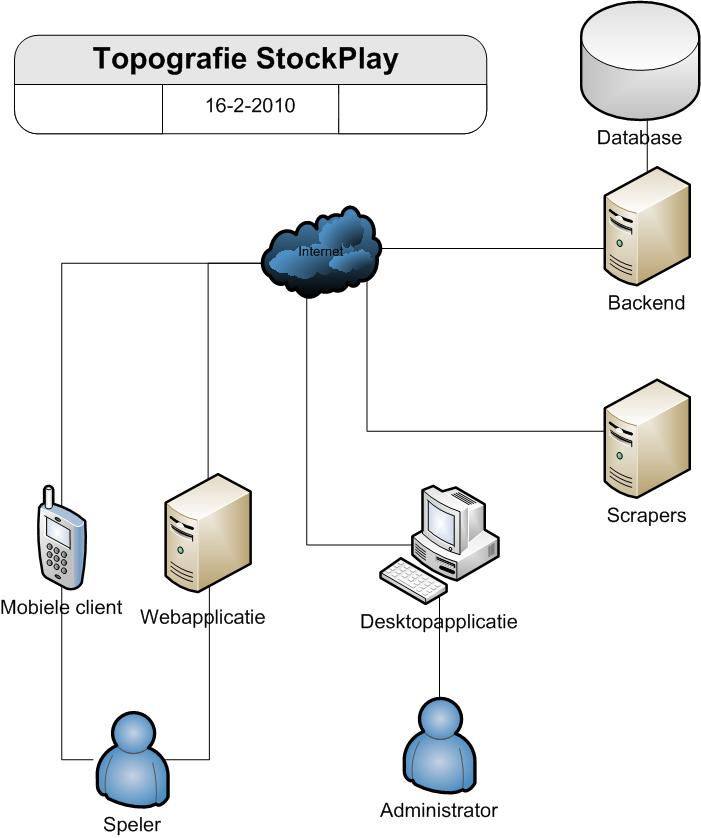
\includegraphics[width=0.5\textwidth]{images/ontwerp/topografie}
	\caption{Topografie van de verschillende systemen.}
\end{figure}

\subparagraph{Scrapers}
StockPlay gebruikt de echte re\"ele beurs, waardoor de koersen van deze effecten moeten dus periodiek worden opgehaald om het spel te laten werken. Hiervoor maken we gebruik van in Perl geschreven scrapers die vanaf enkele vooraf bepaalde internetsites de koersen extraheren. (zoals \makeurl{De Tijd}{http://www.tijd.be/beurzen/euronext-brussel/continumarkt} of \makeurl{Beursduivel}{http://www.beursduivel.be/koersen-belmid.index}).
De opgehaalde informatie wordt vervolgens doorgestuurd naar de backend dewelke deze koersinformatie vervolgens opslaat in de database.

\subparagraph{Atrifici\"ele intelligentie}

Dit zijn computergestuurde spelers, die via het backend-protocol rechtstreeks communiceren met de backend om zo een competitieve medespeler te vormen.


\subsection{Uitwerking User interfaces}

\subsubsection{Webapplicatie}

\begin{figure}[h!]
	\centering
		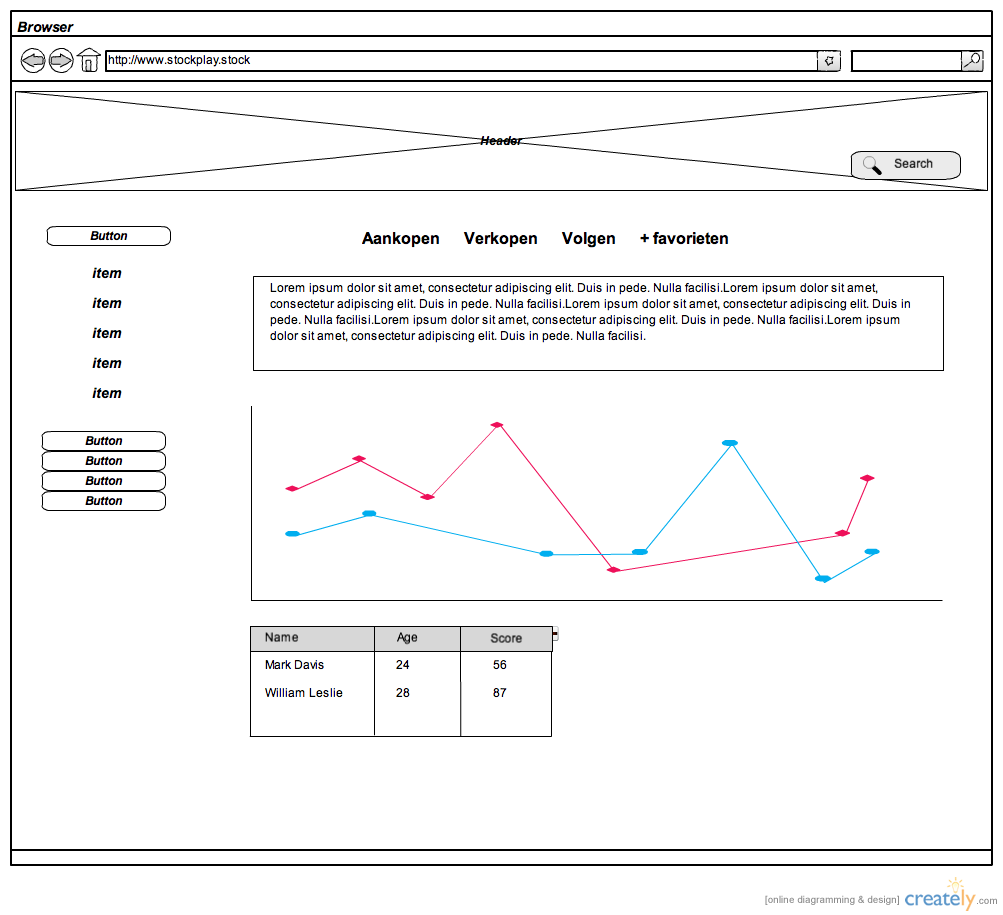
\includegraphics[width=0.5\textwidth]{images/ontwerp/screenshot_website}
	\caption{Layout van de website.}
\end{figure}

Deze interface wordt gebruik om deel te nemen aan het spel. Een gebruiker surft hierbij naar de server die de interface host, en krijgt zo de spelomgeving te zien, dit zonder eerst aan bepaalde softwarevereisten (zoals een Java runtime) te moeten voldaan hebben. Een deel van de functionaliteit is beperkt tot geregistreerde gebruikers.

\paragraph{De algemene overzichtspagina}
Deze pagina geeft de gebruiker een zicht over:
\begin{itemize_compact}
	\item{de huidige waarde van de aangekochte effecten en de meer- of minwaarde op de aankoopprijs}
	\item{zijn cashpositie}
	\item{het totaal van zijn cashpositie en de huidige waarde van de effecten}
	\item{het huidige rendement}
	\item{een grafiek met een overzicht van hun rendement ten opzichte van het gemiddeld rendement, beste rendement, enz.}
	\item{het algemeen klassement en eventuele tussenklassementen}
\end{itemize_compact}

\paragraph{Portfolio}
Vervolgens kan de gebruiker zijn portfolio bekijken, en daar volgende informatie uit halen:
\begin{itemize_compact}
	\item{een overzicht van het portfolio van de gebruiker}
	\item{de effecten momenteel in bezit, aankoopprijs (per stuk en in totaal), huidige koers, rendement en winst/verlies op het aandeel}
\end{itemize_compact}

\paragraph{Overzicht beschikbare effecten}
Er is ook een pagina die een zicht biedt op alle effecten aanwezig in het spel.
\subparagraph{Filters} Om het overzicht te behouden voorziet dat overzicht in verschillende filters:
\begin{itemize_compact}
	\item{per beurs}
	\item{per type (aandeel, tracker, ...)}
	\item{per index}
	\item{per naam}
	\item{aandelen die als favoriet zijn gekenmerkt door de gebruiker}
	\item{per prijs}
	\item{per volume}
\end{itemize_compact}
\subparagraph{Details per effect}Per aandeel kan vervolgens doorgeklikt worden naar een overzichtspagina, die de volgende informatie biedt:
\begin{itemize_compact}
	\item{grafiek met koers}
	\item{hoog/laag van de dag}
	\item{huidige koers}
	\item{openingskoers}
	\item{verschil}
	\item{omzet}
	\item{mogelijkheid om te kopen/te verkopen}
\end{itemize_compact}

\paragraph{Transactiegeschiedenis}De gebruiker kan ook een overzicht bovenhalen waarop zijn transactiegeschiedenis zichtbaar is. 
\subparagraph{Details per transactie}Ook hier kan men steeds doorklikken naar een detailpagina in kwestie:
\begin{itemize_compact}
	\item{het tijdstip}
	\item{het effect}
	\item{het type transactie}
	\item{het aantal}
	\item{de kostprijs voor de transactie}
	\item{de winst/verlies door transactie}
	\item{totaal van uw portefeuille}
\end{itemize_compact}
\subparagraph{Filters}Het overzicht kan worden behouden met behulp van volgende filters:
\begin{itemize_compact}
	\item{enkel aankopen/verkopen}
	\item{enkel met winst/verlies}
\end{itemize_compact}

\paragraph{Klassementen}Er zijn ook verschillende klassementen aanwezig:
\begin{itemize_compact}
	\item{meest aangekochte aandelen}
	\item{meest verkochte aandelen}
	\item{spelers top 20 (waarde Portfolio)}
	\item{spelers top 20 (puntentotaal)}
\end{itemize_compact}

\paragraph{Verhandelpagina effecten}De interface voorziet ook in een pagina om aandelen te kopen of verkopen. Hiervoor zijn verschillende mogelijkheden:
\begin{itemize_compact}
	\item{de prijs die je biedt voor het aandeel. Pas als het aandeel die koers bereikt wordt het aandeel effectief aangekocht}
	\item{de hoeveelheid aandelen die je wenst aan te kopen}
	\item{de max. geldigheidsduur van dit order (1 uur/dag/week/maand)}
\end{itemize_compact}
Tijdens de aankoop krijgt de gebruiker een overzicht van de totale kostprijs en de verschillende taksen die erop staan.

\subsubsection{Desktopapplicatie}
Deze applicatie voorziet in het beheer van het hele systeem. De beheerder logt daarvoor in met behulp van zijn eID.
De desktopapplicatie is opgesplitst in drie grote componenten.

\paragraph{Systeemstatus}Het laatste grote deel van de applicatie biedt een overzicht van de systeemstatus. Daarbij kan de beheerder het volgende ondernemen:
\begin{itemize_compact}
\item{status van de componenten (scraper, database, website, ...) en starten/stoppen/herstarten van degene die dit aankunnen.}
\item{statistieken bekijken}
	\begin{itemize_compact}
	\item{aantal ingeschreven gebruikers sinds de start}
	\item{aantal gebruikers online}
	\item{aantal connecties per tijdseenheid op de backend}
	\item{aantal transacties per tijdseenheid}
	\item{aantal (succesvol/gefaalde/...) gescrapede aandelen per tijdseenheid}
	\end{itemize_compact}
\end{itemize_compact}

\begin{figure}[h!]
	\centering
		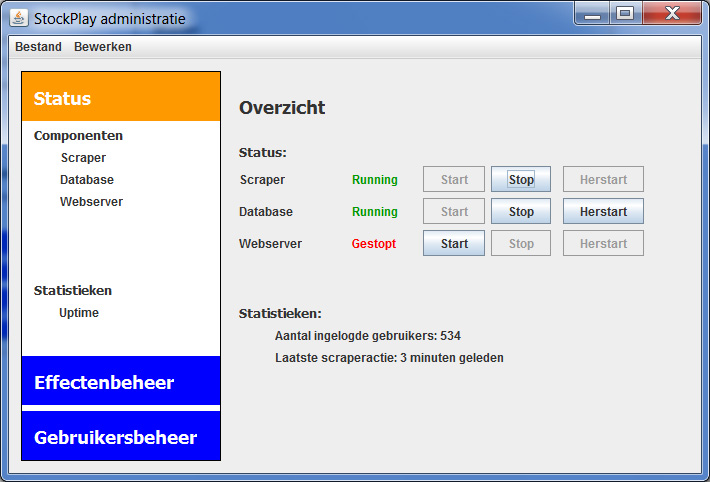
\includegraphics[width=0.5\textwidth]{images/ontwerp/screenshot_app_status}
	\caption{Screenshot van concept statuspagina.}
\end{figure}

\paragraph{Effectenbeheer}Er is ook een overzicht van de effecten voorzien, die de volgende functionaliteit biedt:
\begin{itemize_compact}
	\item{aanduiden van welke effecten moeten gescraped worden, welke effecten zichtbaar zijn bij de spelers}
	\item{schorsen van handel in een effect}
	\item{wijzigen van de gescrapede gegevens}
	\item{overzicht van de aanwezigheid in portefeuilles bij spelers}
\end{itemize_compact}

\begin{figure}[h!]
	\centering
		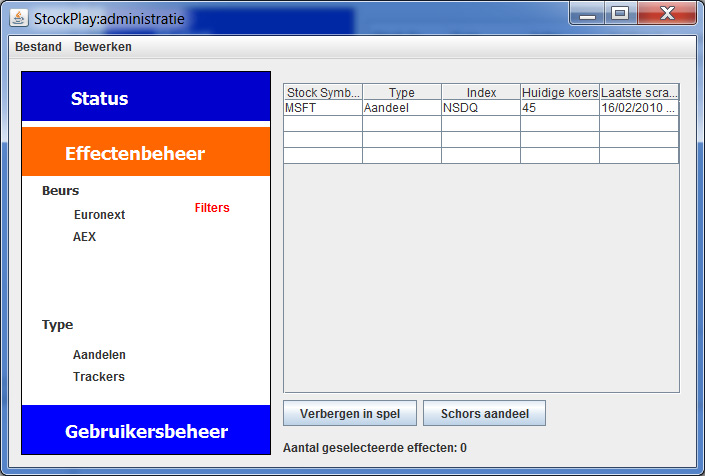
\includegraphics[width=0.5\textwidth]{images/ontwerp/screenshot_app_effecten}
	\caption{Screenshot van concept effectenbeheer.}
\end{figure}

\paragraph{Gebruikersbeheer}Enerzijds is er het overzicht van de gebruikers. Per gebruiker zijn de volgende beheersopdrachten mogelijk: 
\begin{itemize_compact}
	\item{wijzigen van een gebruiker}
	\item{verwijderen van een gebruiker}
	\item{aanpassen van Portfolio: kopen/verkopen van effecten}
	\item{de hoeveelheid cash van de gebruiker aanpassen}
\end{itemize_compact}

\begin{figure}[h!]
	\centering
		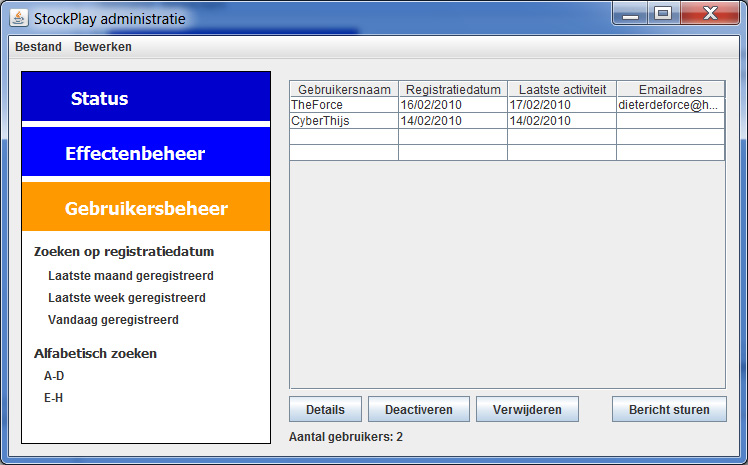
\includegraphics[width=0.5\textwidth]{images/ontwerp/screenshot_app_gebruikers}
	\caption{Screenshot van concept gebruikersbeheer.}
\end{figure}


%
% Technisch
%

\section{Technisch ontwerp}

\subsection{Hergebruik}

\subsubsection{Backend protocol}

Om toegang te krijgen tot de backend vanuit de verschillende andere delen van het project (zoals de scraper, AI, of interfaces) moesten we op zoek gaan naar een goed communicatieprotocol dat aan verschillende vereisten moet voldoen:
\begin{itemize}
\item{\emph{Taalonafhankelijk}: aangezien de interfaces met behulp van verschillende programmeertalen gerealiseerd worden, moet de interface toegankelijk zijn vanuit verschillende programmeertalen.}
\item{\emph{Lichtgewicht}: voor de communcicatie met onze mobiele interface, moet de gegenereerde data compact gehouden worden.}
\item{\emph{Toegankelijk}: de interfaces moeten toegankelijk zijn vanaf een andere machine dan die waar de backend op draait.}
\end{itemize}

Zo hebben we een aantal protocollen overwogen:
\begin{itemize_compact}
\item{een eigen binair protocol}
\item{RMI}
\item{SOAP}
\item{XML-RPC}
\end{itemize_compact}

Het binair protocol viel nogal snel af, aangezien lastig is om te implementeren, relatief foutgevoelig is, en geen garanties biedt qua toegankelijkheid. RMI was ons niet toegestaan te gebruiken, waardoor nog twee kandidaten overbleven: SOAP en XML-RPC. Bij het vergelijken van beide bleek SOAP nogal zwaarwichtig te zijn, en bovendien veel te uitgebreid voor onze (relatief eenvoudige) eisen.

Zo hebben we uiteindelijk gekozen voor het XML-RPC protocol. Dit is een lichtgewicht Remote Procedure protocol, die methodeaanvragen en -antwoorden verpakt in XML-data en ze als POST request verstuurd over het HTTP protocol (zie ook bijlage \ref{chap:xml-rpc} voor de specificaties).
Het protocol voldoet ook aan de opgestelde eisen: aangezien het verder bouwt op het bestaande HTTP-protocol kan het gebruik maken van diens mogelijkheden (zoals compressie en encryptie) en kan het (indien een specifieke bibliotheek niet beschikbaar zou zijn) eenvoudig verwerkt worden met behulp van reeds bestaande HTTP- en XML-bibliotheken. Bovendien verschilt de communicatie niet van regulier HTTP-verkeer waardoor de toegankelijkheid in gelimiteerde netwerkomgevingen ook toeneemt.

Voor de programmeertalen die we gaan gebruiken bij het implementeren bleken er reeds verschillende bibliotheken beschikbaar te zijn, wat het gemak van gebruik opnieuw verhoogt. Een opsomming van de specifieke bibliotheken die we zullen gebruiken om informatie te versturen en ontvangen over het XML-RPC protocol:
\begin{itemize_compact}
\item{\textbf{Perl}: \makeurl{RPC::XML}{http://search.cpan.org/dist/RPC-XML/}}
\item{\textbf{C\#}: \makeurl{XML-RPC.NET}{http://www.xml-rpc.net/}}
\item{\textbf{Java}: \makeurl{Apache XML-RPC}{http://ws.apache.org/xmlrpc/}}
\item{\textbf{Java ME}: \makeurl{kXML-RPC}{http://kxmlrpc.sourceforge.net/}}
\end{itemize_compact}

Deze keuzes zijn eveneens voorzichtig gemaakt. Zo kent Perl nog verschillende andere XML-RPC bibliotheken (zoals de compactere \makeurl{XML::RPC}{http://search.cpan.org/dist/XML-RPC/} bibliotheek). Initi\"eel hadden we ook gekozen voor deze XML::RPC module (onder andere wegens het beperktere aantal afhankelijkheden), maar naar mate het project vorderde liepen we tegen enkele limitaties van die bibliotheek (zoals gebrek aan compressie), en ook enkele structurele problemen. Zo probeert de XML::RPC module dynamisch-getypeerde Perl variabelen automagisch te gebruiken binnen het sterk-getypeerde XML-RPC protocol, wat verschillende keren vervelende bugs veroorzaakte. Daarom zijn we omgeschakeld naar RPC::XML, waar sterk-getypeerde variabelen ge\"emuleerd worden door gebruik van expliciete conversiefuncties die instaan voor de omzetting van de al-omvattende Perl variabelen, naar speciefieke RPC::XML dataobjecten (zoals RPC::XML::int, RPC::XML::struct, etc).
Om XML-RPC te gebruiken in Java zijn er ook alternatieven, zoals de \makeurl{Redstone XML-RPC bibliotheek}{http://xmlrpc.sourceforge.net/} die afviel door zijn beperkte featureset, en door het feit dat het al enige tijd niet meer onderhouden was (dit in tegenstelling tot de Apache libraries, die ook een heel actieve community kent).
Voor C\# en Java.ME hebben we geen alternatieve bibliotheken gevonden.

\subsection{Dynamische grafieken}

Op de internetwebsite zullen we een extra module ontwikkelen waarin grafieken dynamisch gemanipuleerd kunnen worden. De gebruikers zullen met eenvoudige muishandelingen andere grafische weergaven van de grafieken kunnen opvragen, zonder de pagina te herladen. Hiervoor zal gebruik gemaakt worden van de interpreter taal Javascript en de javascript bibliotheken \makeurl{JQuery}{http://jquery.com/} en \makeurl{Flot}{http://code.google.com/p/flot/}. JQuery is benodigd om de Flot bibliotheek werkend te krijgen en kunnen we ook op andere plaatsen op de website gebruiken. Deze bibliotheek gaat wat extra functies aan de HTML-elementen hangen en geeft ons eenvoudige middelen om met AJAX extra informatie op te halen.

We gebruiken Flot omdat aan deze bibliotheek nog acief ontwikkeld wordt. Alsook is ze heel eenvoudig gehouden en kan je er makkelijk op voortbouwen. Je kan er op voortbouwen door de ingebouwde events op te vangen en door gebruik te maken van de ingebouwde plugin functionaliteit. Er is ook ondersteuning voor datumweergave en er zijn plugins waarmee je een selectievenster op de grafiek kan activeren (om in te zoomen) en om de grafiek te kunnen verslepen.
De grafieken worden getekend met een combinatie van HTML elementen en het CANVAS element. De HTML elementen kunnen we gemakkelijk vormgeven met CSS. Canvas wordt ge\"emuleerd in Internet Explorer. Alsook kunnen we de grafieken van deze bibliotheek op een eenvoudige manier vullen met JSON.

\subsection{Hardware}

\todo{Een vermelding van de mobiele interface}
